\documentclass{beamer}
\usetheme{ODK}
\usepackage{tikz}

\usepackage[utf8]{inputenc}
\usepackage{graphicx}
\graphicspath{{../../../Proposal/Pictures/}}

\makeatletter
\newskip\@bigflushglue \@bigflushglue = -100pt plus 1fil
\def\bigcenter{\trivlist \bigcentering\item\relax}
\def\bigcentering{\let\\\@centercr\rightskip\@bigflushglue%
\leftskip\@bigflushglue
\parindent\z@\parfillskip\z@skip}
\def\endbigcenter{\endtrivlist}
\makeatother

\author{Nicolas M. Thiéry}
\title{Wrap up}

\begin{document}

\begin{frame}{Time to wrap up}
  \centerline{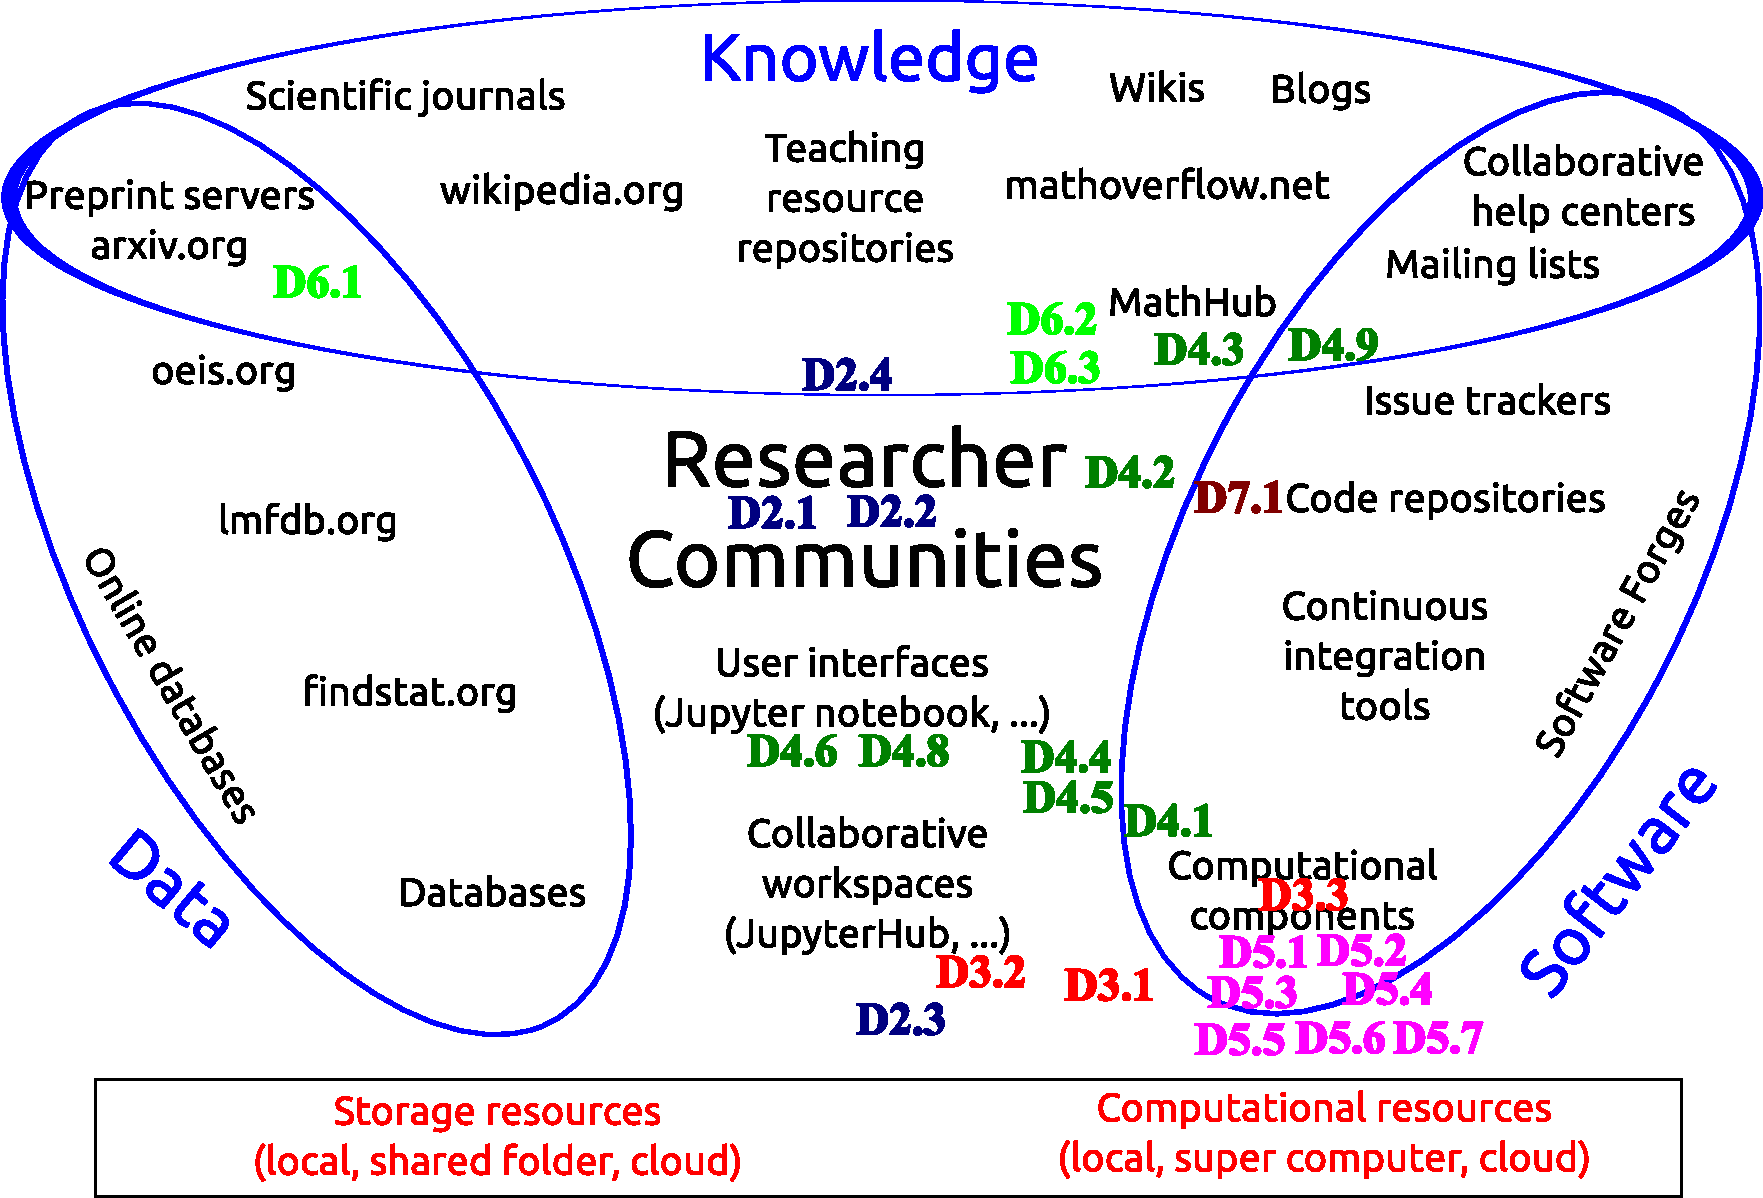
\includegraphics[height=.85\textheight]{TheBigPictureDeliverables.pdf}}
\end{frame}

\begin{frame}{Time to wrap up}
  \begin{itemize}
  \item The consortium has come up together as an effective team\\
    Spawning many cross system collaborations
    \pause\bigskip
  \item The Jupyter stack has been booming\\
    Adoption and deployment at scale
    \pause\bigskip
  \item VREs based on ecosystem have matured or appeared:
    \begin{itemize}
    \item SageMathCloud, ...
    \item try.jupyter.org, mybinder.org, ...
    \item jupyter.math.cnrs.fr, jupyter.u-psud.fr, ...
    \item notebooks.azure.com, ...
    \end{itemize}
    \pause\bigskip
  \item Some decade old issues are close to resolution\\
    e.g. packaging, portability
    \pause\bigskip
  \item Shall we claim all the credit? \pause \textbf{No, just a fraction of it!}\\\pause
    Thanks to: strong ecosystem, strong communities, openness
  \end{itemize}
\end{frame}

\end{document}
